\documentclass[10pt]{article}
\usepackage[margin=0.75in]{geometry}
\usepackage{lmodern}
\usepackage{booktabs,graphicx,amsmath,microtype}
\usepackage[hidelinks]{hyperref}
\usepackage{titlesec}
\titlespacing*{\section}{0pt}{6pt}{3pt}
\titleformat{\section}{\normalsize\bfseries}{\thesection}{0.6em}{}
\setlength{\parskip}{2pt}
\begin{document}

\begin{center}
{\large\bfseries Does chain-of-thought still protect against J-space ablation when problems get hard?}\\[2pt]
CS 2881 Homework 0 \,$\cdot$\, \today\ \,$\cdot$\, code: \texttt{github.com/pgrindehollevik-harvard/cs2881}
\end{center}

\section{Hypothesis (pre-registered before any experiment; tag \texttt{prereg-v1})}
Gurnee et al.\ (2026) show that a model's ``J-space'' can be deleted: at every token
position, across a band of middle layers, one zeroes the residual stream's projection
onto the $k{=}10$ most active Jacobian-lens directions. In their frontier models this
deletion destroys internal multi-step reasoning, spares shallow skills, and, most
strikingly, spares GSM8K \emph{when the model writes its reasoning out}. Written
chain-of-thought appears to substitute for the internal workspace. We tested whether
that protection survives on a much smaller model, \texttt{Qwen/Qwen3-4B}, and whether
it survives increasing difficulty. \textbf{H1} (replication): on GSM8K, chain-of-thought
protects more than direct answering does, beyond what matched random damage explains.
Formally, the random-differenced protection
$P_D=[R(\text{CoT},J)-R(\text{dir},J)]-[R(\text{CoT},\text{rand})-R(\text{dir},\text{rand})]$
is positive (predicted magnitude $\ge +0.15$), where $R$ is accuracy retention
(ablated/clean). \textbf{H2} (extension): the protection \emph{erodes} as problems get
harder (GSM8K $\to$ MATH-500 $\to$ AIME; within MATH-500, levels 1$\to$5). Rationale:
externalization has limited bandwidth, and each written step of a harder problem still
demands more internal workspace. Falsification criteria, sample sizes, floor rules, and
a hypothesis-blind calibration gate were frozen in \texttt{docs/PREREGISTRATION.md}
before any run. Every later departure is timestamped in \texttt{docs/DEVIATIONS.md}.

\section{Experiment design}
The design is a grid: two prompting modes (chain-of-thought vs.\ direct answer, same
sampling settings) $\times$ three conditions (clean, J-space ablation, control ablation)
$\times$ three datasets (GSM8K $n{=}150$; MATH-500 stratified 30 per level; AIME
2024+2025, all 60 problems). The control ablation is the design's backbone: deleting
ten directions damages any network, so at every (position, layer) we instead remove an
\emph{exactly equal-norm} component along random directions. Whatever survives the
$P_D$ subtraction is therefore specific to the J-space, not generic damage.
A stop-gate stands in front of the main grid. Before it may run, the ablation must
reproduce, on this model, both signatures the paper found: (1) a positive-control
reasoning drop that is significant (exact McNemar) and at least $2\times$ the
matched-random drop, with output degeneration below 10\%; and (2) selectivity, meaning
ordinary next-token prediction on held-out wikitext survives (top-1 agreement with the
clean model above 0.80; our pre-registered quantification of the paper's selectivity
finding, whose exact values appear only in its Fig.~22 graphic). Ablation strength (the
layer band and $k$) is calibrated only against these gauges. The calibration never sees
a CoT-vs-direct comparison, so it cannot be tuned toward the hypothesis.

\section{Experimental details}
The companion repository provides the lens but no ablation code, so we implemented the
intervention as forward hooks. At each (position, band layer): compute readout logits
$\mathrm{lm\_head}(\mathrm{rmsnorm}(J_\ell h))$; take the top-10 token ids, recomputed
independently per position and layer; exempt any id in the clean model's top-10
next-token predictions (a parallel clean stream over the same tokens supplies these);
form directions $v_t=J_\ell^{\top}(\gamma\odot W_U[t])$; remove their joint projection
by a regularized batched solve. Ablation applies to the prompt and to every generated
token. The lens is the pre-fitted \texttt{neuronpedia/jacobian-lens} artifact, fit on
this exact checkpoint. We validated it before use: it beats a logit-lens baseline at
ranking silent multi-hop intermediates (pass@5 $0.41$ vs $0.37$; pass@1 $0.20$ vs
$0.19$), though not on arithmetic order-of-operations readouts at rank 1; the
pre-registered gate (win on either eval) passed. The paper reports its workspace band
as percent depth, so we transferred it by proportion: candidates
$\{14\text{--}24,\,14\text{--}31\}$ of Qwen3-4B's 36 blocks, with a light band
14--19. Compute was one M4 Pro (48\,GB, MPS); ablated decode ran 3.4--7.2 tok/s across
calibration rungs (median ${\approx}6$; the ablated pass runs two streams plus
per-layer readouts). Generation is chunk-resumable with 64-token persistence, which
mattered: macOS update preparation repeatedly SIGKILLed the process (90\,s lifetimes at
the worst), costing wall-clock but, by construction, no data. Grading uses
\texttt{math-verify} on the last \verb|\boxed{}|; no-answer, truncation, degeneration,
and wrong-answer are tracked as separate classes. Seven unit tests certify the
intervention: exact identity when disabled, projections verifiably removed, the
exemption rule honored, per-slot norm matching, seeded determinism, and chunked equal
to unchunked.

\section{Experimental results}
\textbf{Calibration.} The paper's positive control (``multihop'': silent two-hop
factual composition, e.g.\ legs of the animal that spins webs) proved unusable here:
clean Qwen3-4B scores only 0.42 where frontier models are near ceiling. This is itself
a small-model datum. The pre-registered fallback control (``order-ops'': arithmetic
order-of-operations completions, clean 0.745) was used instead. All four rungs then
\emph{failed} the stop-gate, so the main grid did not run on the stock lens:

\begin{center}\small
\begin{tabular}{lcccc}
\toprule
Rung & J drop (pts) & random drop & wikitext top-1 (J / rand) & gate\\
\midrule
14--24, $k{=}10$ & $-16.4$ ($p{=}.004$) & $-9.1$ & $0.62\,/\,0.79$ & fail\\
14--31, $k{=}10$ & $-18.2$ & $-9.1$ & $0.58\,/\,0.73$ & fail\\
14--24, $k{=}5$ & $-14.5$ & $-5.5$ & $0.61\,/\,0.82$ & fail\\
14--19, $k{=}10$ (light) & $-16.4$ ($p{=}.012$) & $\phantom{-}0.0$ & $0.66\,/\,0.84$ & fail\\
\bottomrule
\end{tabular}
\end{center}

Read the table as two separate findings. First, the J-directions are causally real on
Qwen3-4B. In the light band, deleting them costs 16 points on the control while
exactly norm-matched random deletion costs \emph{nothing} ($n{=}55$ paired items,
exact McNemar $p{=}.012$), and outputs stay coherent (degeneration 3\%). Second, the
directions are not \emph{selective}: 34--42\% of ordinary next-token predictions
change, whereas the paper finds ablation leaves ``the bulk of ordinary text prediction
intact'' (\S3.5.2). The damage always spills into everyday prediction.
The pre-registered contingency then applied: the stock lens targets the final layer,
while the paper prefers a penultimate target to avoid last-block artifacts, so we
refit a penultimate-target lens and re-ran the ladder. Fit size was $n{=}32$ prompts
rather than the registered $n{\approx}100$, because 17 hours of MPS backward passes
made $n{=}100$ infeasible (deviation 4, whose interpretation rule was committed before
the re-run). All four rungs failed again, and diagnostically so: the refit lens's
``J-directions'' behaved identically to the random control (drops $10.9$ vs $10.9$;
$14.5$ vs $12.7$). Selectivity worsened at the $k{=}10$ rungs (0.45--0.56) and stayed
comparable at the gentler rungs (0.62--0.68), never approaching the 0.80 gate. This is
what estimation noise dominating a small fit should look like, which would in turn
corroborate the stock lens's J-vs-random gap as real structure; deviation 4's
registered confound means we treat that reading as suggestive rather than established.

\begin{center}
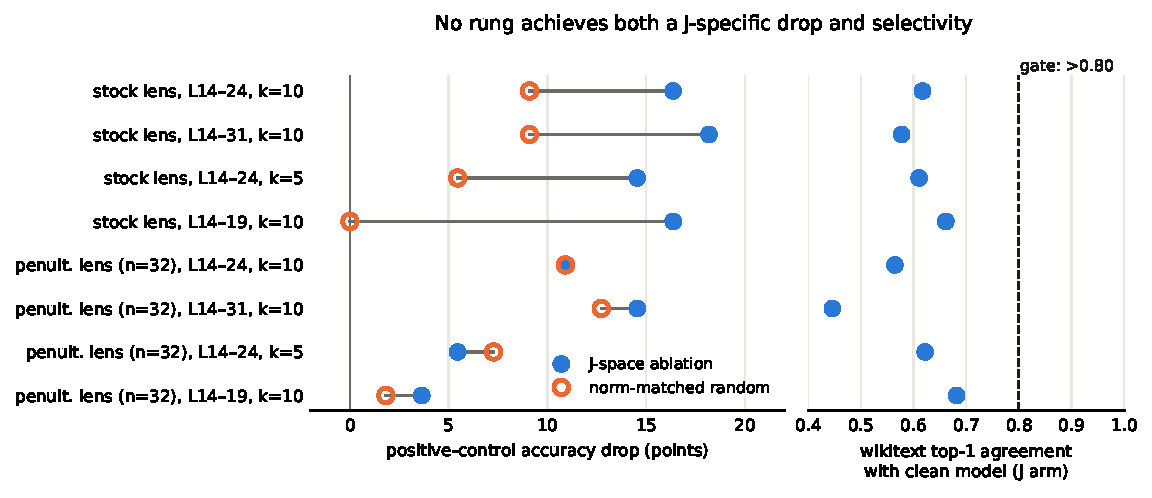
\includegraphics[width=\linewidth]{../results/figures/ladder.pdf}
\end{center}

\section{Analysis of results}
\textbf{Verdict.} H1 and H2 could not be answered on this model, and that is the
finding. The pre-registered precondition for interpreting any CoT-vs-direct comparison
(an ablation that is J-specific \emph{and} spares ordinary prediction) was not
achievable at any of eight settings across two lenses. We report the negative
replication rather than an uninterpretable grid. \textbf{What is positively
established:} (i) the Jacobian lens transfers to Qwen3-4B as a readout, beating the
logit lens at surfacing silent multi-hop intermediates; (ii) its directions are
causally load-bearing, since the light band shows a 16-point J drop against a zero
norm-matched-random drop with coherent outputs; (iii) what fails to transfer is the
paper's selectivity signature, the separation of workspace from ordinary prediction.
\textbf{Two readings remain.} (a) Small models route ordinary next-token prediction
\emph{through} their verbalizable representations, so the workspace/automatic
separation is an emergent property of scale. This fits the paper's own Haiku 4.5
warning and our finding that clean Qwen3-4B scores only 0.42 on two-hop silent
composition. (b) Lens estimation quality at 4B (the stock lens early-stopped at
$n{=}479$, with a final-layer target) smears workspace directions with
general-prediction components. Our refit could not settle (b) at a feasible fit size,
so it is reported as unresolved, not refuted. \textbf{Next with more compute:} run the
same pre-registered ladder on Qwen3-14B and 32B, for which pre-fitted lenses exist.
Reading (a) predicts the gate starts passing with scale; reading (b) predicts it keeps
failing. Also: a full-budget penultimate lens, and thinking-mode traces. All code,
prompts, seeds, the full 8-rung calibration records (including per-item outcomes), and
the crash-tolerant pipeline are in the repository for exact reuse. The main grid's
records intentionally do not exist.

\end{document}
